\documentclass{ximera}


%\addPrintStyle{../..}

\begin{document}
	\author{Bart Lambregs}
	\xmtitle{Het referentiestelsel}{}
    \xmsource\xmuitleg


Elk bewegend systeem wordt beschreven ten opzichte van een \textbf{referentiestelsel}. Deze omvat een assenstelsel met een oorsprong (= het \textbf{referentiepunt}).
Binnen dit referentiestelsel worden de vectoriële grootheden beschreven waaruit de kinematica is opgebouwd. 
 
Als je een vogel ziet vliegen kan je deze beweging op verschillende manieren beschrijven: de vogel kan \textit{stijgen} of een \textit{duikvlucht} nemen. De vogel kan \textit{omdraaien} of -indien het een kolibri is- misschien zelfs \textit{blijven hangen}. Om deze bewegingen kwantitatief en nauwkeurig te bespreken kies je een referentiestelsel en coördinaatassen. Op die manier krijgt de vogel een positievector die de positie aangeeft, een snelheidsvector die de snelheid aangeeft, ... 

De keuze van het referentiestelsel is altijd relatief. Toch is het erg belangrijk om telkens duidelijk te maken van waaruit een beweging beschreven wordt.
Stel je voor dat je op dit moment gedreven natuurkunde aan het studeren bent aan een bureau en je houdt je pen op \textit{ooghoogte}, hoe 'hoog' bevindt je pen zich dan? Meet je dit vanaf je tafelblad, de vloer, het straatniveau, het aantal meters boven de zeespiegel, ...? In welke eenheid meet je dit? Wat is je eenheidsvector en in welke richting kies je de positieve as? 

Meestal wordt geopteerd voor een referentiestelsel waarvoor de 'waarnemer' stilstaat. % footnote bewegende referentiestelsels --> speciale relativiteit  
In onderstaand voorbeeld van het voetbalveld is de positie \(\vec{r}\) van de voetballer duidelijk verschillend is naargelang het referentiepunt.
Voor een toeschouwer in het publiek staan beide referentiestelsels stil, bijgevolg is de snelheid \(\vec{v}\) voor beiden dezelfde.


\begin{center}
\begin{minipage}[t]{0.70\textwidth}
\begin{image}[\linewidth]
	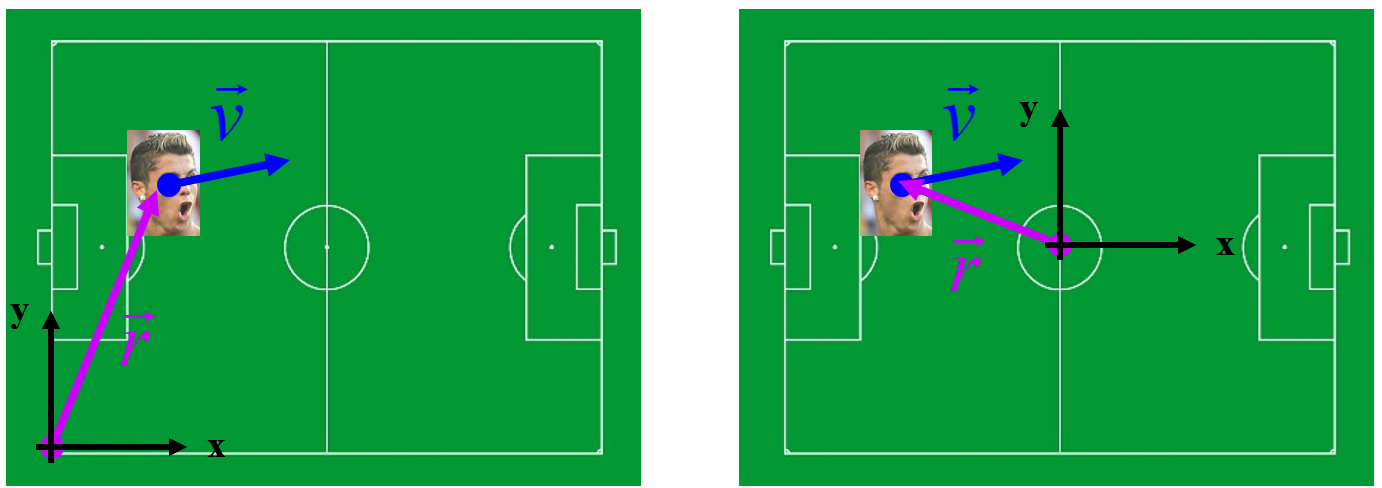
\includegraphics{referentiestelsels}
% Uit ppt Vincent, IK WIL AFBEELDING GROTER MAAR LUKT ME NIET.
\end{image}
\end{minipage}
\end{center}
\captionof{figure}{Twee verschillende referentiestelsels}


\begin{exercise}
De kolibri in onderstaande foto blijft ter plekke in de lucht hangen onder de bloem. Geef twee referentiestelsels waarin deze vogel \textbf{niet} stilstaat. 

\begin{center}
\begin{minipage}[t]{0.30\textwidth}
\begin{image}[\linewidth]
	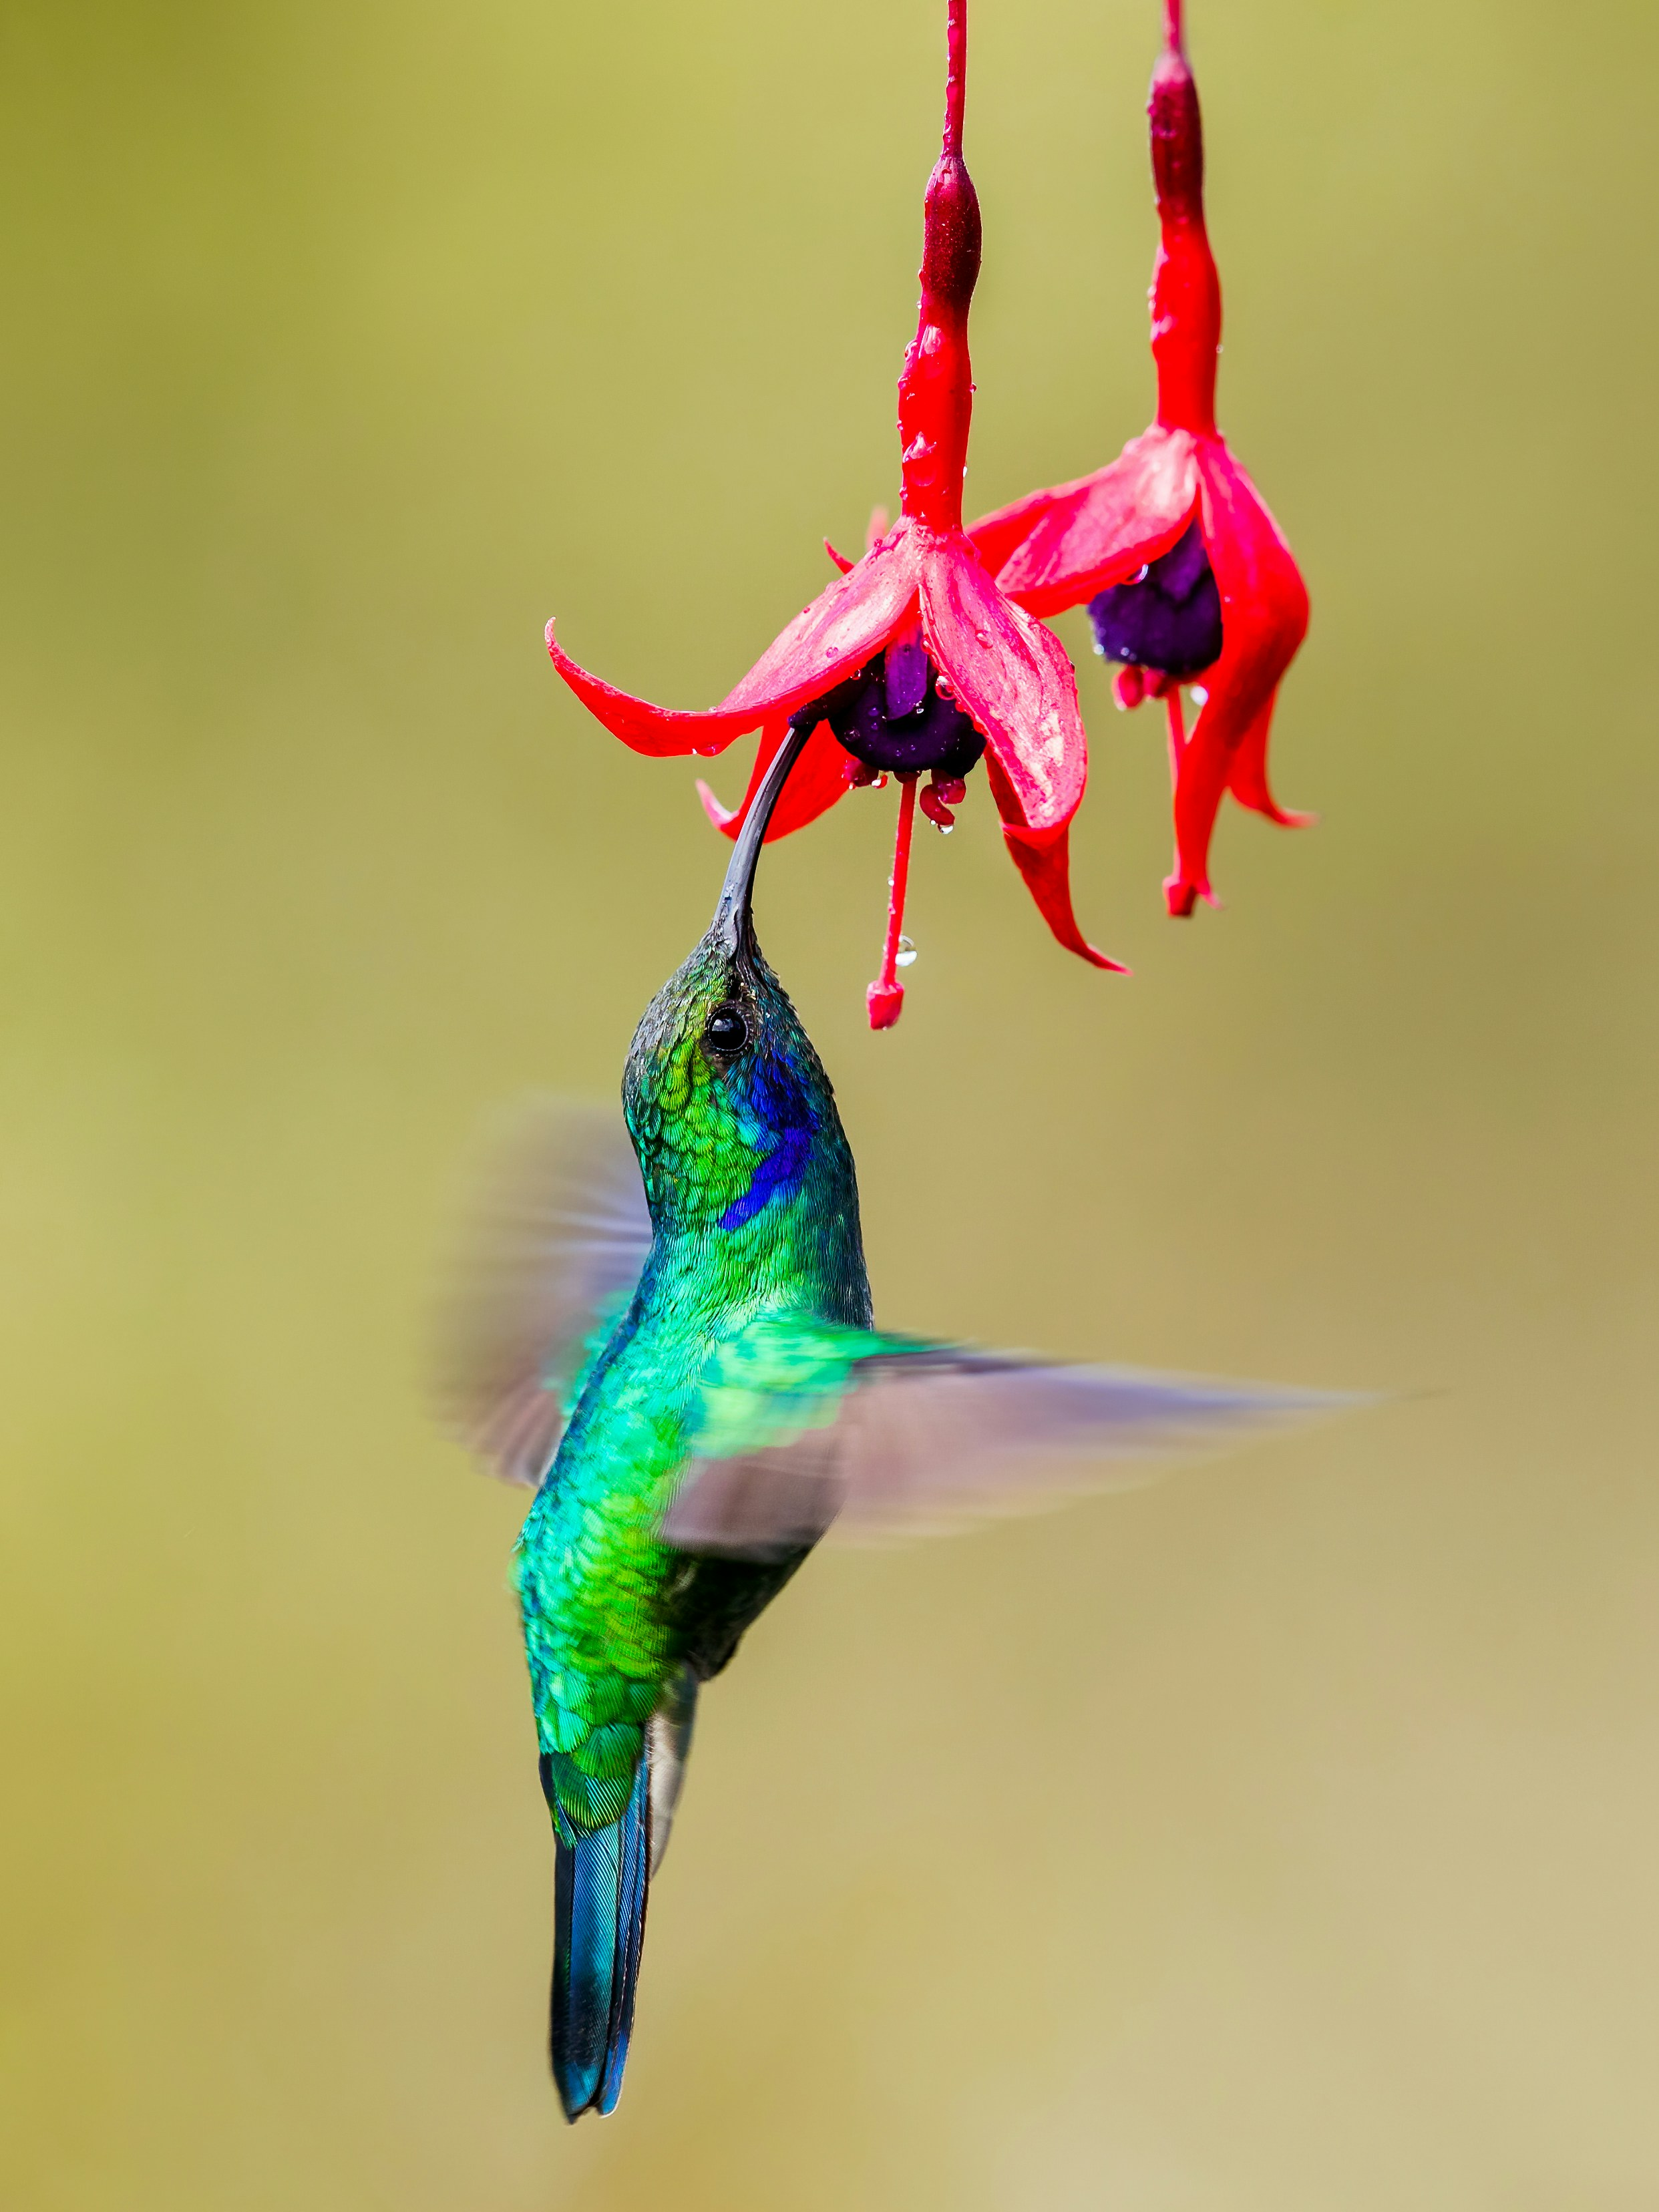
\includegraphics{kolibri}
% Bron: https://unsplash.com/photos/green-and-black-humming-bird-flying-p-DDK9lOmmE 
\end{image}
\end{minipage}
\end{center}


\begin{oplossing}\nl
\begin{itemize}
\item Een referentiestelsel met de kern van de aarde als oorsprong. (De kolibri draait nu rond de as van de aarde...)
\item Een referentiestelsel met de zon als middelpunt (De kolibri draait nu ook rond de zon...)
\end{itemize}

\end{oplossing}

\end{exercise}


\end{document}




